% -----------------------------------------------------------------------------
% Páginas Web
% -----------------------------------------------------------------------------

\chapter{Desenvolvimento de Páginas Web}
\label{chap:devWeb}

O sétimo capítulo do presente trabalho tem como objetivo a implementação de páginas Web utilizando a biblioteca de componentes previamente desenvolvida. As seções a seguir detalharão o processo de criação das interfaces de usuários desenvolvidas nesta fase: telas de listagem de componentes e tela de \textit{login}.

\section{Telas de listagem de componentes}
\label{sec:listaComponentes}

Como forma de garantir um ponto focal para a documentação da biblioteca de componentes, as primeiras páginas Web implementadas foram aquelas que apresentavam os componentes criados. A \autoref{fig:listComponentsButton} apresenta uma das páginas de apresentação de componente: a página do componente \textit{dito-button}.

A idéia inicial era de que, em cada container de listagem de componentes, fosse apresentado o componente em si juntamente do código-fonte necessário para a sua renderização. Pelo motivo do prazo de entrega para o presente trabalho não o permitir, tal funcionalidade não foi contemplada na versão inicial destas páginas.

Desejava-se que todas as páginas criadas fossem baseadas na biblioteca de componentes, entretanto tanto o cabeçalho quanto a seção de navegação da página não foram definidos por ela em sua primeira versão. Faz-se necessária uma refatoração do código-fonte, no futuro, para abstrair tais elementos para componentes da biblioteca.

\begin{figure}
  \begin{center}
	  \frame{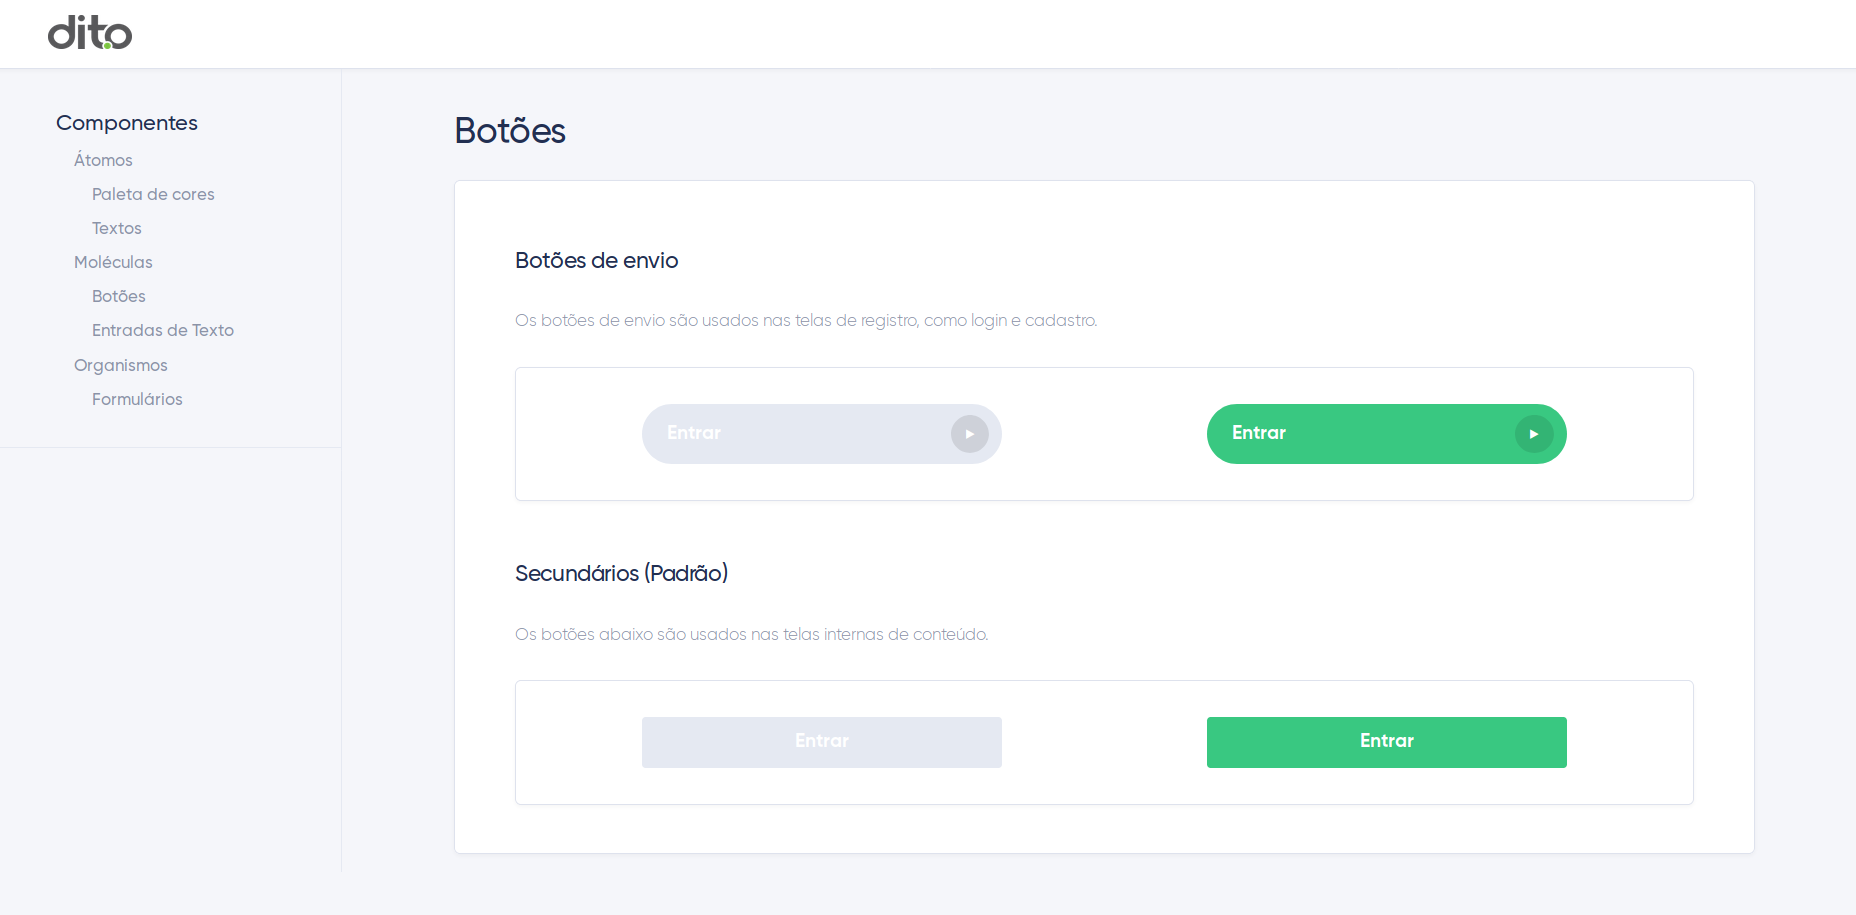
\includegraphics[width=\linewidth]{./04-figuras/07_paginas_web/lista-componentes.png}}
	\end{center}
  \caption{Página de apresentação do componente \textit{dito-button}}
  \fonte{Próprio autor}
  \label{fig:listComponentsButton}
\end{figure}

\section{Tela de \textit{login}}
\label{sec:telaLogin}

A primeira página implementada para o projeto \textit{DitoFeras} foi a página de \textit{login}. A \autoref{fig:loginPage} ilustra o resultado final de sua implementação.

\begin{figure}
  \begin{center}
	  \frame{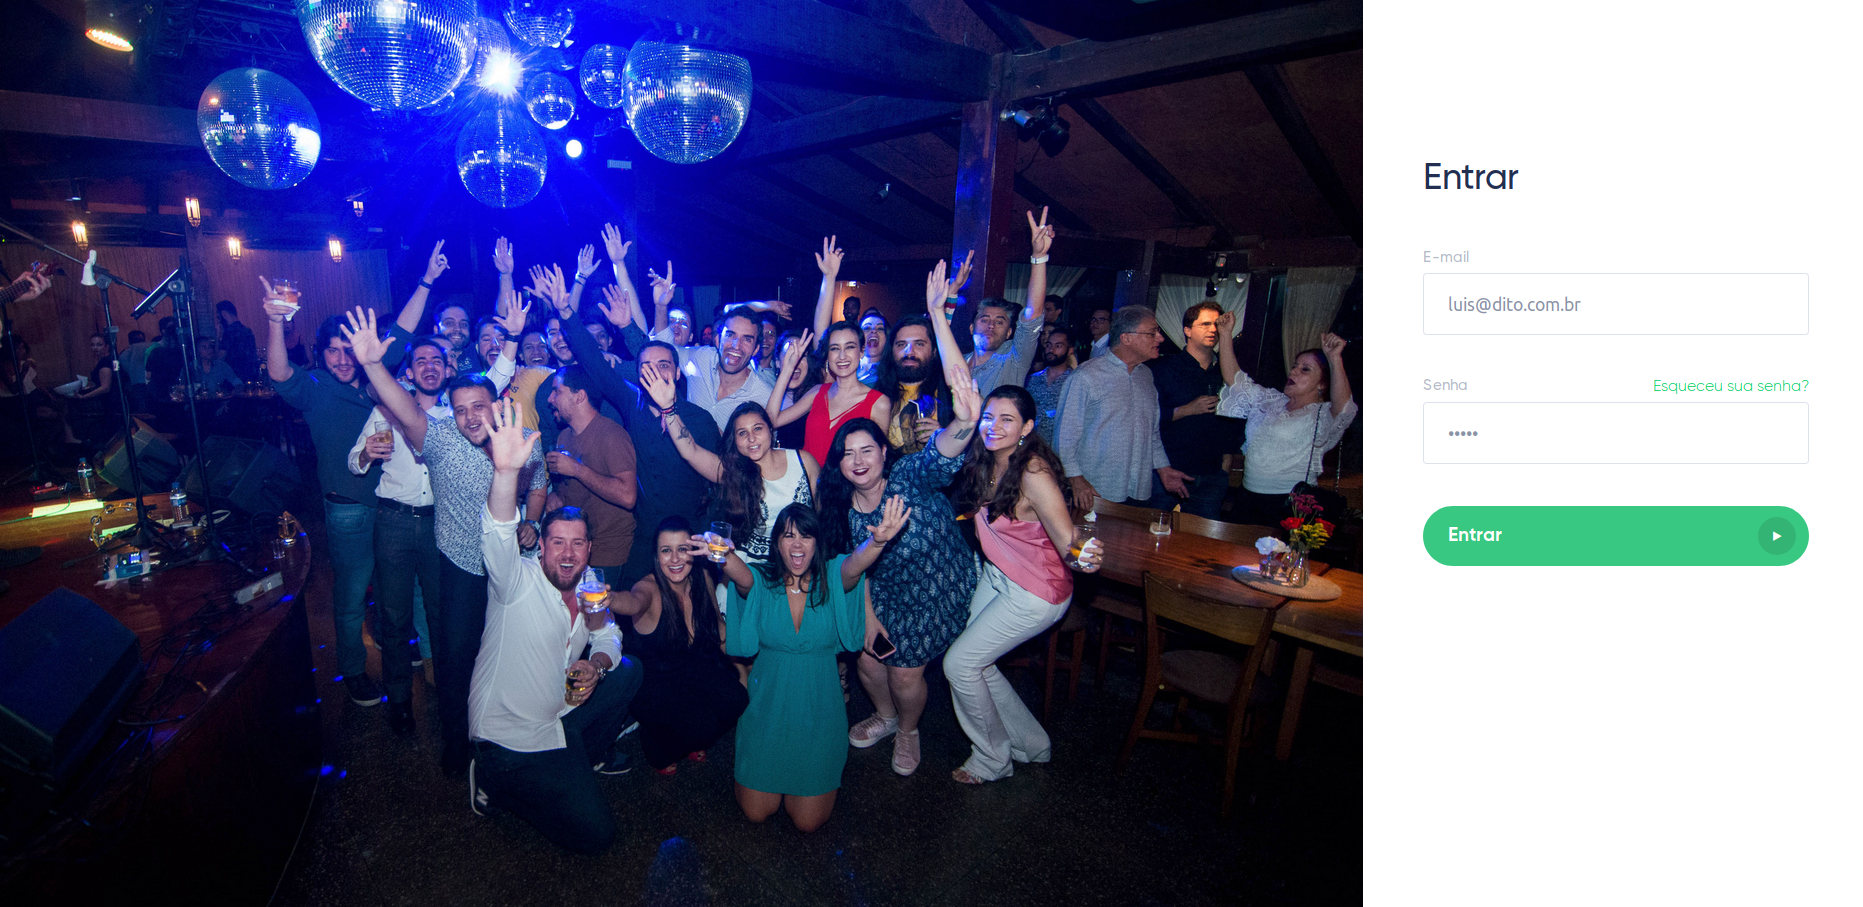
\includegraphics[width=\linewidth]{./04-figuras/07_paginas_web/login.png}}
	\end{center}
  \caption{Página de \textit{login} do sistema \textit{DitoFeras}}
  \fonte{Próprio autor}
  \label{fig:loginPage}
\end{figure}

Diferentemente das páginas de listagem de componentes, esta foi construida utilizando única e exclusivamente os componentes da biblioteca. A \autoref{fig:loginCode} apresenta todo o código-fonte necessário para a construção da página de \textit{login}. Fica evidente o quão simples é o desenvolvimento de novas interfaces de usuários baseadas em componentes previamente implementadas. Muito do comportamento da página acaba já sendo implementado pelos componentes envolvidos, restando assim apenas o esforço de posiciona-los adequadamente ao longo da interface.

\begin{figure}
  \begin{center}
	  \frame{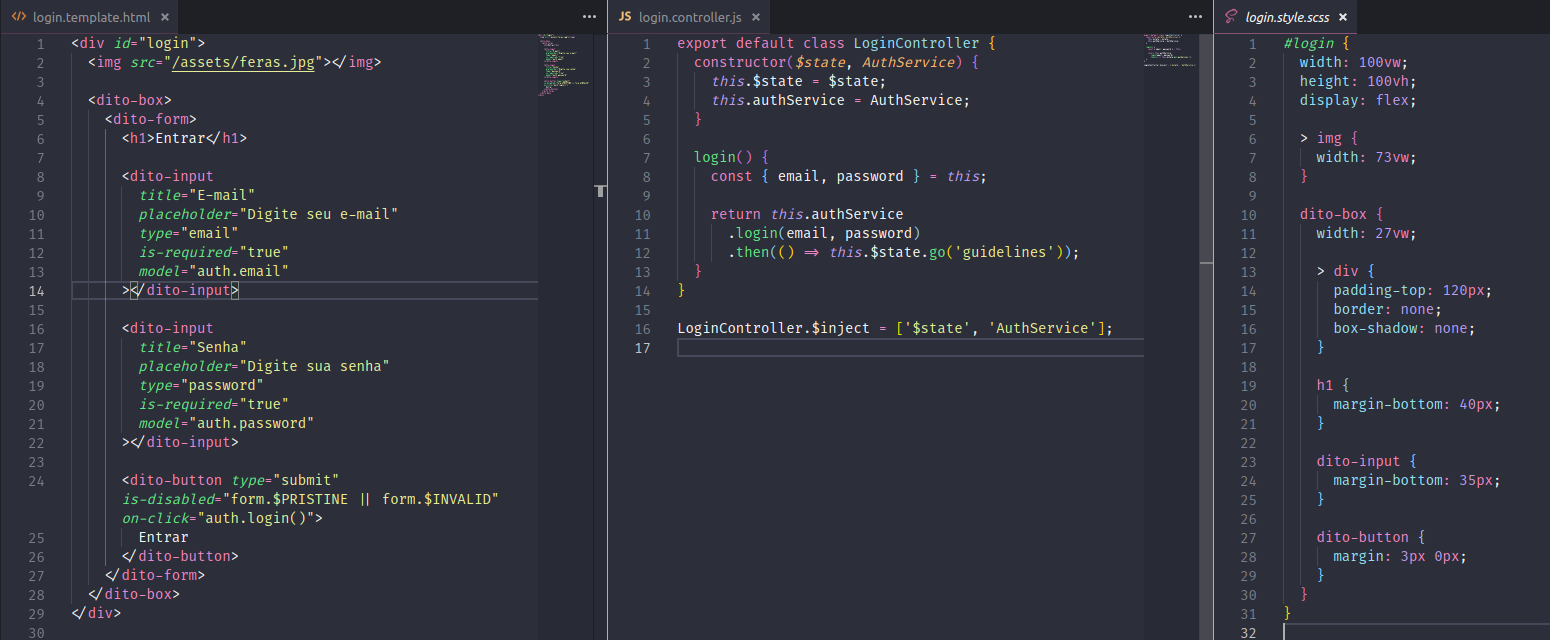
\includegraphics[width=\linewidth]{./04-figuras/07_paginas_web/login-code.png}}
	\end{center}
  \caption{Código-fonte da página de \textit{login} do sistema \textit{DitoFeras}}
  \fonte{Próprio autor}
  \label{fig:loginCode}
\end{figure}

Restava ainda a página de listagem de funcionários da empresa, proposta como um dos primeiros entregáveis do projeto. Novamente, pelo fator prazo de entrega, essa funcionalidade também não foi implementada nesta primeira versão.

No capítulo seguinte é discutida, detalhadamente, a avaliação dos resultados obtidos através do presente trabalho.
